\tikzset{
  enpd/base/.style={
    ->,
    font=\small,
    node distance=3em and 8em
  },
  enpd/group/.style={
    draw,
    rectangle,
    minimum height=3.2em,
    minimum width=7em,
    align=center,
    fill=white
  },
  enpd/store/.style={
    rectangle,
    minimum height=3.2em,
    minimum width=7em,
    align=center,
    fill=white,
    draw=none,
    path picture={
      \draw (path picture bounding box.north west) -- (path picture bounding box.north east);
      \draw (path picture bounding box.south west) -- (path picture bounding box.south east);
    }
  },
  enpd/process/.style={
    draw,
    circle,
    minimum size=5.4em,
    align=center,
    fill=white
  },
  enpd/hotspot/.style={
    enpd/process,
    postaction={
      dashed,
      pattern=north west lines,
      pattern color=red!60
    }
  },
  enpd/context/.style={
    draw,
    dashed,
    inner sep=1pt,
    rounded corners=5pt,
    pattern=north east lines
  },
  enpd/label/.style={
    fill=white,
    opacity=0.65,
    text opacity=1,
    inner sep=1pt
  },
  enpd/flow-label/.style={
    enpd/label,
    opacity=1
  },
  enpd/flow/.style={thick},
  enpd/flow-bi/.style={enpd/flow,<->},
  enpd/flow-uni/.style={enpd/flow,->}
}
% \enpdStore[tikz options]{ref}{label}{count}{energy}
\newcommand{\enpdStore}[5][]{%
  \node[enpd/store,#1] (#2) {#3};%
  \node[enpd/label,anchor=south east,yshift=1pt] at (#2.north east) {n=#4};%
  \def\enpdtmp{#5}\ifx\enpdtmp\empty\else
    \node[enpd/label,anchor=north,yshift=-1pt] at (#2.south) {[$#5$]};%
  \fi
}
% \enpdStoreAt[tikz options]{ref}{label}{count}{energy}{at}
\newcommand{\enpdStoreAt}[6][]{%
  \node[enpd/store,#1] (#2) at (#6) {#3};%
  \node[enpd/label,anchor=south east,yshift=1pt] at (#2.north east) {n=#4};%
  \def\enpdtmp{#5}\ifx\enpdtmp\empty\else
    \node[enpd/label,anchor=north,yshift=-1pt] at (#2.south) {[$#5$]};%
  \fi
}
% \enpdProcess[tikz options]{ref}{label}{energy}
\newcommand{\enpdProcess}[4][]{%
  \node[enpd/process,#1] (#2) {#3};%
  \def\enpdtmp{#4}\ifx\enpdtmp\empty\else
    \node[enpd/label,anchor=north,yshift=-1pt] at (#2.south) {[$#4$]};%
  \fi
}
\newcommand{\enpdHotspot}[4][]{%
  \node[enpd/hotspot,#1] (#2) {#3};%
  \def\enpdtmp{#4}\ifx\enpdtmp\empty\else
    \node[enpd/label,anchor=north,yshift=-1pt] at (#2.south) {[$#4$]};%
  \fi
}
% \enpdGroup[tikz options]{ref}{label}{count}
\newcommand{\enpdGroup}[4][]{%
  \node[enpd/group,#1] (#2) {#3};%
  \node[enpd/label,anchor=south east,yshift=1pt] at ([xshift=2ex,yshift=2ex]#2.north east) {n=#4};%
  \begin{scope}[on background layer]%
    \draw[fill=white] ([xshift=2ex,yshift=2ex]#2.north west) rectangle ([xshift=2ex,yshift=2ex]#2.south east);%
    \draw[fill=white] ([xshift=1ex,yshift=1ex]#2.north west) rectangle ([xshift=1ex,yshift=1ex]#2.south east);%
  \end{scope}%
}
% \enpdContext[tikz options]{ref}{nw}{se}{label}{count}
\newcommand{\enpdContext}[6][]{%
  \begin{scope}[on background layer]%
    \coordinate (nw) at ($(#3) + (-4ex,4.5ex)$);%
    \coordinate (se) at ($(#4) + (4ex,-4.5ex)$);%
    \node[enpd/context,fit=(nw)(se),#1] (#2) {};%
  \end{scope}%
  \node[enpd/label,anchor=north west] at (#2.north west) {#5};%
  \node[enpd/label,anchor=north east] at (#2.north east) {n=#6};%
}

Deploying data\-/centred systems responsibly requires balancing different priorities, such as effectiveness, data privacy and environmental sustainability.
Understanding and tracking energy consumption throughout the system architecture is essential for making informed decisions about resource allocation and environmental impact.
While Data Processing Diagrams have proven effective for modelling data flows and privacy safeguards, they do not visualise energy consumption.
This paper introduces Energy Processing Diagrams, an extension of Data Processing Diagrams, that integrates energy information.
These diagrams provide a shared visual and analytical language that helps software engineers design more sustainable software projects in collaboration with stakeholders.
They enable teams to track energy flows, compare architectures, identify energy\-/intensive components and reason about trade-offs.
Through a case study, we show how sustainability considerations can be integrated into architectural thinking from the earliest design phases by making energy data visible and actionable.

\section{Introduction}
As software systems grow in scale and complexity, their environmental footprint shifts from a marginal operational concern to a primary design constraint. However, integrating sustainability into the software development life cycle remains a significant challenge. Recent studies highlight that software developers are often hindered by a lack of empirical knowledge and a deficit of actionable tools to measure or mitigate software energy consumption effectively~\cite{pinto2017energy}.

While traditional hardware-centric energy metrics exist, they rarely provide software developers with the information needed to understand how specific architectural choices or data flows contribute to the overall footprint of their system. To address these impacts, practitioners often look towards Life Cycle Assessment (LCA) methodologies. Yet, applying LCA to the rapidly evolving domain of software is complicated by the methodological diversity within the environmental sciences. The landscape of assessment has become increasingly fragmented, leading to what has been described as an \emph{alphabet soup}~\cite{guinee2018digesting} of LCA modes, including attributional (ALCA), consequential (CLCA) and various explorative varieties, such as prospective or scenario-based LCA.
This methodological complexity makes it challenging for software engineers to decide between modelling a system as a static snapshot of environmental impacts or as a dynamic system that changes with architectural modifications.

The challenge has become particularly pronounced with the proliferation of Artificial Intelligence (AI) systems, which often rely on energy\-/intensive computational pipelines involving cloud services and resource\-/intensive algorithms~\cite{berthelot2024estimating,lannelongue2021green}. Current estimates suggest that the energy use of the Information and Communications Technology (ICT) sector already accounts for approximately \qtyrange{2}{3}{\percent} of global greenhouse gas emissions, which is a figure that is expected to rise significantly as AI integration accelerates~\cite{guldner2024development}. This trend is particularly concerning, given the growing tension between privacy preservation and energy efficiency, where techniques like encryption or decentralised processing, while crucial for data protection, can significantly increase computational overhead and energy consumption~\cite{bieker2025data}.

Recent research highlights the need for standardised energy disclosure for AI systems, drawing parallels with energy ratings commonly found on household appliances~\cite{luccioni2024light}. Furthermore, studies show that even seemingly small digital activities, such as email usage, can accumulate significant environmental impacts when scaled across millions of users~\cite{siy2025elitter}. This has led to growing concerns about the intended and unintended consequences of energy consumption disclosure on user behaviour and decision-making~\cite{klesel2026good}.

\subsection{Bridging the architectural gap}
Traditionally, privacy and environmental sustainability are treated as separate concerns. Data Processing Diagrams (DPDs) were developed as a suitable modelling technique that extends Data Flow Diagrams (DFDs) to provide a standardised, shared language for multidisciplinary teams~\cite{bieker2025data,yourdon1979structured}. By maintaining a high abstraction level, DPDs allow engineers, legal experts and educators to reason about privacy tactics, such as encryption and pseudonymisation, from the earliest design phases. However, a system's energy consumption remains out of scope for DPDs, making it difficult for stakeholders to identify how specific design choices affect a system's energy footprint.

The Green Software Measurement Model (GSMM) provides a comprehensive reference framework for assessing soft\-ware-induced energy consumption through standardised metrics and technical measurement setups~\cite{guldner2024development}. While the GSMM is effective for detailed technical evaluation, it operates primarily at the component level, lacking integration with high-level architectural models. This creates a critical gap between early-stage design decisions and their environmental implications. Since software decisions directly influence hardware energy use, energy efficiency must be recognised as a design problem, not just an operational one~\cite{hindle2012green}.

\subsection{Research contributions and approach}
This paper introduces EnPDs to bridge the gap between architectural modelling and energy measurement. EnPDs extend the structural modelling of DPDs by integrating energy-related data, as suggested by the GSMM framework. These diagrams function as analytical models, where architectural components are annotated with actual or estimated energy profiles, enabling multidisciplinary teams to visualise energy costs and identify energy \emph{hotspots} within proposed systems.

The development of EnPDs was motivated by the lack of existing tools that effectively bridge the gap between sustainability goals and architectural decision-making. While various approaches address either energy measurement or system modelling in isolation, we found no comprehensive method that integrates both perspectives in a way that supports sustainable design from the earliest stages. EnPDs fill this gap by providing a practical framework for \emph{green by design} approaches, enabling developers to consider environmental impact alongside other system requirements.

The framework is validated through a case study of the mAIndmap educational platform, where we demonstrate how EnPDs help identify energy hotspots and highlight architectural trade-offs. The rest of the paper thereafter discusses related work, limitations and future directions.

\section{Foundational principles}
EnPDs represent a synthesis of two distinct domains: the structural modelling of software architectures and technical assessment of software-induced energy consumption.
By combining the visual clarity of DPDs with the standardised metrics of the GSMM, EnPDs provide a framework for reasoning about sustainability during the architectural design phase.
While DPDs excel at modelling privacy safeguards, they lack the vocabulary to express the energy implications of these measures. For instance, end-to-end encryption ensures data confidentiality but increases processing overhead. Similarly, data minimisation techniques reduce privacy risks but may require additional computational steps to implement. EnPDs bridge this gap by allowing software developers and stakeholders to quantify and visualise the energy cost of software system components, enabling informed trade-offs between security and sustainability.

\subsection{Architectural modelling}
\begin{figure}[t]
  \centering
  \begin{minipage}[b]{0.23\textwidth}
    \centering
    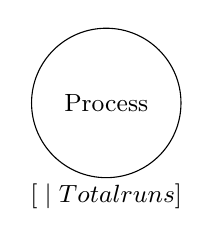
\begin{tikzpicture}[enpd/base,scale=0.8]
      \enpdProcess{process}{Process}{\si{\watthour\per\run} \mid \text{Total runs}}
    \end{tikzpicture}
    \par\medskip
    \centering\footnotesize (a) Process node.
  \end{minipage}%
  \hfill
  \begin{minipage}[b]{0.23\textwidth}
    \centering
    \begin{tikzpicture}[enpd/base,scale=0.8]
      \enpdHotspot{hotspot}{Hotspot}{\si{\watthour\per\run} \mid \text{Total runs}}
    \end{tikzpicture}
    \par\medskip
    \centering\footnotesize (b) Hotspot process.
  \end{minipage}%
  \hfill
  \begin{minipage}[b]{0.23\textwidth}
    \centering
    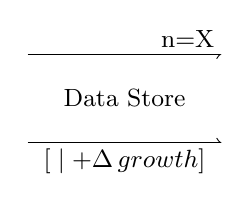
\begin{tikzpicture}[enpd/base,scale=0.8]
      \enpdStore{store}{Data Store}{X\,\si{\giga\byte}}{\si{\watthour} \mid +\Delta\si{\watthour}\,\text{growth}}
    \end{tikzpicture}
    \par\medskip
    \centering\footnotesize (c) Data store node.
  \end{minipage}%
  \hfill
  \begin{minipage}[b]{0.23\textwidth}
    \centering
    \begin{tikzpicture}[enpd/base,scale=0.8]
      \enpdGroup{group}{Group}{N}
    \end{tikzpicture}
    \par\medskip
    \centering\footnotesize (d) Grouped entities.
  \end{minipage}
  % Four figures arranged horizontally, illustrating the core elements of the Energy Processing Diagram notation, labelled (a) to (d). Figure (a) shows a standard Process node containing metrics for Watt-hours per run and total runs. Figure (b) shows a Hotspot node with the same metrics, but highlighted to indicate a hotspot. Figure (c) shows a Data Store node displaying a capacity of X gigabytes and metrics for Watt-hours and delta Watt-hour growth. Figure (d) shows a Grouped entities node with N elements.
  \caption{Core elements of the Energy Processing Diagram notation.}\label{fig:elements}
\end{figure}

DPDs provide a foundation for modelling modern, complex data processing systems through several core structural elements. Figure~\ref{fig:elements} shows how these elements are visualised in EnPDs:
\begin{itemize}
  \item\emph{processes} (the computational operations that transform or handle data),
  \item\emph{hotspots} (energy\-/intensive components, visually dis\-tin\-guished with a dashed red pattern),
  \item\emph{data stores} (where data is held at rest) and
  \item\emph{a group of entities} (a logical collection of external actors).
\end{itemize}

This abstraction is critical for multidisciplinary teams, as it provides a shared language that allows software developers and non-technical stakeholders to identify energy\-/intensive components and evaluate optimisation strategies, such as computational offloading or model compression, consistently across the system.

A central innovation in DPDs is the use of \emph{context boundaries}, which delineate organisational, legal and physical domains. In the context of EnPDs, these boundaries help visualise where energy consumption occurs within the system architecture. By placing processes and data stores within specific boundaries, software developers and stakeholders can better understand the energy implications of architectural decisions, such as whether to process data locally or in the cloud.
This is particularly valuable in distributed AI systems, where computational load and its associated energy costs might be distributed across different parts of the system, helping stakeholders identify which energy-saving opportunities are most actionable within their sphere of influence.

\subsection{Measurement integration}
In an EnPD, every process or data store is treated as a potentially measured object with a specific goal.
To move beyond high-level overviews, EnPDs adopt some approaches from the GSMM, which provides a structured reference for assessing the resource efficiency of software products. While the GSMM is designed for detailed energy assessments, EnPDs are intended for early-stage architectural design where estimated values are often more practical and sufficient for comparative analysis. The framework remains compatible with empirical data when they become available, allowing for increasing precision as the design progresses.

This model designates energy (measured in Watt-hours $[\si{\watthour}]$ or Joules $[\si{\joule}]$) as the primary metric, potentially supplemented by secondary indicators, like runtime (\si{\second}), hardware utilisation (CPU/GPU, in \si{\percent}) and network throughput (\si{\mega\byte}).
By standardising these metrics and units, EnPDs ensure that the annotations within a diagram are comparable across different architectural iterations.

The transition from DPDs to EnPDs requires careful consideration of both architectural design and energy impact assessment. While DPDs provide the structural foundation for displaying data flows between actors, processes and storage units, EnPDs extend this by incorporating energy-related annotations that help reason about the environmental implications of design choices. This integration enables stakeholders to make informed decisions about energy efficiency during the early design phases, when architectural changes are most cost-effective to implement.

\section{The Energy Processing Diagram framework}
The EnPD framework extends DPDs by integrating energy data into architectural models. While maintaining DPDs' focus on information flow, EnPDs provide a structured method for evaluating the energy implications of data processing, storage and transfer. This extension allows stakeholders to consider energy efficiency as a first-class constraint during the earliest stages of system design.

A critical scoping decision in the EnPD framework is the exclusion of production and deployment costs, also known as \emph{embodied energy}. Although the manufacturing and transport of hardware represent a significant portion of a system's total environmental footprint, EnPDs are specifically intended to be a tool for those involved in system architecture design. By focusing exclusively on \emph{operational energy} (the consumption driven by software components and data transit) the EnPD framework isolates the variables that system architecture designers can directly influence. This ensures that the model remains a clear reflection of architectural efficiency rather than a hardware life cycle assessment.

To maintain clarity in multi-stakeholder settings and ensure that diagrams remain actionable, EnPDs adhere to the following conventions:
\begin{itemize}
  \item \emph{Context boundaries.} In the EnPD framework, the concept of boundaries is retained to define the structural and administrative environments of system components, though they do not explicitly imply energy responsibility or accountability. This allows teams to distinguish between local, cloud and third-party environments without complicating the model with attributional logic.
  \item \emph{Data flow representation.} Real-world network interactions often involve asymmetrical energy costs for uploading and downloading data. However, at the architectural design level, capturing this granularity often introduces additional complexity. EnPDs utilise an aggregated bidirectional metric for data flows, which can be expressed in two ways. The first notation, $[\si{\watthour\per\transfer} \mid \text{Total transfers}]$, is intended for analytical modelling, where identifying the frequency of high-cost transfers is necessary to evaluate optimisation strategies, like batching. Alternatively, the $[\si{\watthour}]$ notation may be used for high-level summaries, providing a simplified, comparable value representing the total cost of a communication link without detailing the underlying frequency.
  \item \emph{Process annotation.} Computational operations are treated as measured objects, with the annotation drawn directly beneath the component. Similar to data flows, designers can choose between two modes. The $[\si{\watthour\per\run} \mid \text{Total runs}]$ notation is the preferred style for optimisation tasks, as it allows designers to distinguish between an inefficient algorithm and a high-demand service. For instances where a process is a constant background task or where the frequency is irrelevant to the specific architectural comparison, the simplified $[\si{\watthour}]$ notation may be utilised.
  \item \emph{Data storage metrics.} Storage units are annotated with their energy consumption in \si{\watthour}, shown below the component. The physical size of the data store is indicated in the top-right corner using the notation `n=X \si{\giga\byte}'. This separation of concerns allows designers to focus on both the storage requirements and their associated energy costs. The energy annotation can represent either the total annual cost of maintaining the stored data or, when relevant, the energy cost of data growth over time (e.g., $[\si{\watthour} \mid +\Delta\si{\watthour}\,\text{growth}]$). This approach enables stakeholders to evaluate both the immediate and long-term energy use implications of data storage decisions.
  \item \emph{Identification and visualisation of energy hotspots.} To support rapid deci\-sion-making, EnPDs make use of a structured pipeline.
  First, the total energy consumption for each individual component and data flow is calculated by multiplying its unit energy cost by its expected execution frequency.
  Second, a pool of hotspot candidates is established by filtering these results to include only \emph{actionable} nodes and data flows (the ones that the stakeholders have architectural control over).
  For instance, highly intensive cloud components, such as AI model training machines, are deliberately excluded from this candidate pool if they cannot be directly altered by the system design team.
  Third, the final hotspots are determined by isolating the candidates that exceed a predefined accepted threshold value that depends on the task associated with that node or data flow.
  These definitive hotspots are then visually highlighted using dashed red patterns: processes and data stores are marked with a red dashed background, while data flows are represented with dashed red arrows.
  This systematic filtering provides an immediate cognitive map of energy\-/intensive, addressable components, allowing system designers to quickly identify and prioritise them for refinement.
\end{itemize}

By standardising these conventions, the EnPD framework ensures that energy annotations are not merely decorative but serve as a basis for comparing different architectures. This alignment between measurement and design allows for green software principles to be systematically applied during the earliest stages of the software development life cycle.

\section{Case study: mAIndmap}
Using a case study, we show how EnPDs can support architectural decision-making even before a concrete implementation exists.
We start with a skeleton Data Flow Diagram derived from the project requirements document, annotate it with yearly energy labels based on estimates and then refine the architecture incrementally.
The goal is to make trade-offs visible already during the design phase, while design choices are still open.

NOLAI is an organisation focused on developing AI-driven solutions for educational purposes.
One of their projects, mAIndmap, centres on an AI-assisted tool for vocabulary learning in early primary education (grades~1--3, ages~4--6, in the Dutch education system).
Teachers in these grades use mindmaps to expand children's vocabulary: a central concept is shown with an image in the middle, surrounded by related words and images.
In practice, creating such mindmaps is time-consuming and disrupts the flow of lessons, especially when teachers have to search for age-appropriate illustrations during classes.
The mAIndmap project addresses this by generating the mindmap structure and accompanying images automatically, with the help of several AI components.

\subsection{Baseline: Skeleton DFD}
The proposed architecture relies on two main AI components.
First, a word-embedding model trained on the \emph{BasiLex} corpus~\cite{tellings2014basilex} (\textasciitilde11.5 million words from Dutch primary school reading material) computes semantic similarity and determines word placement in the mindmap.
Second, a text-to-image model generates age-appropriate illustrations in a consistent visual style.
To keep latency low during lessons, images for words likely to arise in grades~1--3 are pre-generated, with missing images generated on demand.

The architecture spans two contexts relevant to this case study: the school environment, which consists of classrooms and infrastructure, and a cloud-based back-end.
The project's design proposal contains a DPD that documents data flows and privacy classifications across these contexts, which serves as the starting point for the design of the skeleton Data Flow Diagram.
After omitting details from the project proposal that are not relevant to the case study, we arrive at the DFD shown in Figure~\ref{fig:dfd}.

\begin{figure}[t]\begin{tikzpicture}[enpd/base]
    % Server context
    \enpdProcess{backend}{Backend}{}
    \enpdProcess[right=of backend]{lm}{Language\\model}{}
    \enpdStore[below=of lm]{localstorelm}{Model\\storage}{\qty{1}{\giga\byte}}{}
    % Cloud context
    \enpdStore[below=10.7em of backend]{imagedb}{Image\\database}{\qty{30}{\giga\byte}}{}
    \enpdProcess[below=of imagedb]{imagegen}{Image\\generation}{}
    \enpdStore[below=of imagegen]{cloudstoreimg}{Model\\storage}{\qty{4}{\giga\byte}}{}
    \enpdProcess[below=of cloudstoreimg]{trainimg}{Model\\training}{}
    \enpdStoreAt{cloudstorelm}{Model\\storage}{\qty{1}{\giga\byte}}{}{imagegen.east -| localstorelm.south}
    \enpdProcess[below=of cloudstorelm]{trainlm}{Model\\training}{}
    % Classroom
    \enpdGroup[above=of backend]{classroom}{Classroom\\context}{10}
    % Contexts
    \enpdContext[pattern color=orange!55]{server}{$(backend.north -| imagedb.west)$}{$(localstorelm.south east)$}{Server}{1}
    \enpdContext[pattern color=blue!35]{cloud}{$(imagedb.north west)$}{$(trainimg.south -| cloudstorelm.east)$}{Cloud}{1}
    % Flows
    \draw[enpd/flow-bi] (classroom.south) -- (backend.north);
    \draw[enpd/flow-bi] (backend.east) -- (lm.west);
    \draw[enpd/flow-uni] (lm.south) -- (localstorelm.north);
    \draw[enpd/flow-uni] (cloudstorelm.north) -- (localstorelm.south);
    \draw[enpd/flow-bi] (backend.south) -- (imagedb.north);
    \draw[enpd/flow-uni] (trainlm.north) -- (cloudstorelm.south);
    \draw[enpd/flow-uni] (imagegen.north) -- (imagedb.south);
    \draw[enpd/flow-uni] (cloudstoreimg.north) -- (imagegen.south);
    \draw[enpd/flow-uni] (trainimg.north) -- (cloudstoreimg.south);
  \end{tikzpicture}%
  % Data Flow Diagram showing the mAIndmap architecture with two main contexts: a school server (orange) and cloud infrastructure (blue). The school context contains a backend process, language model process and model storage (1 GB). The cloud context includes an image database (100k images), image generation process, two model storages (4 GB and 1 GB, respectively) and training processes for both language and image models. A classroom context at the top represents 10 classrooms. Arrows show data flows between components.
  \caption{Skeleton Data Flow Diagram, extracted from the described architecture in the mAIndmap project proposal.}\label{fig:dfd}
\end{figure}

\subsection{Constructing an EnPD from the DFD}
Then, to construct an EnPD from the DFD, we maintain the same structure and add yearly energy labels to components and inter-context data flows.
The model represents a single school, with all energy terms scaled accordingly.
The labels account for baseline infrastructure power, persistent storage, inference workloads and network transfer, using the assumptions summarised in Table~\ref{tab:energy-estimates}.

\begin{table}[H]
  \centering
  \begin{tabular}{lc}
    \toprule
    \multicolumn{1}{c}{Component} & \multicolumn{1}{c}{Cost}    \\
    \midrule
    Mindmap structure size & \qty{10}{\kilo\byte\per\mindmap}   \\
    Generated image size   & \qty{300}{\kilo\byte\per\image}    \\
    Network transfer       & \qty{0.1}{\watthour\per\giga\byte} \\
    Local storage          & \qty{15}{\watt\per\tera\byte}      \\
    Cloud storage          & \qty{5}{\watt\per\tera\byte}       \\
    \bottomrule
  \end{tabular}
  \caption{Baseline assumptions and energy estimates used to calculate energy costs for the mAIndmap components.}\label{tab:energy-estimates}
\end{table}

In the school context, three elements contribute energy: local infrastructure, local language model storage and local language model inference.
We assume an always-on local server with a baseline draw of \qty{10}{\watt}, corresponding to \qty{88}{\kilo\watthour} per year.
Across grades~1--3, we estimate 10 classes per school and 20 lessons per class per year, giving 200 mindmap requests annually.
Language model inference executes locally at \qty{0.1}{\watthour} per mindmap structure.
Its \qty{1}{\giga\byte} local model storage contributes \qty{131}{\watthour} per year.

The cloud environment covers image generation, shared image storage and delivery to schools.
The language model is synchronised once per year, while image retrieval requires a network transfer for every requested image.
If an image is missing from the shared database, it is generated on demand and then retained in storage.
We estimate 15 images per mindmap, yielding 3,000 image retrievals per year across 200 lessons, of which 300 require generation.

The cloud context also contains training and model storage.
Model training is assumed to consume \qty{10}{\kilo\watthour} for the language model and \qty{500}{\kilo\watthour} for the image model.
We deliberately do not consider these nodes as hotspots, as they are not directly actionable for the stakeholders in this case study.
Cloud storage is set to \qty{5}{\watt\per\tera\byte} and cloud image inference to \qty{15}{\watthour} per image, which is lower than the school context, reflecting economies of scale relative to local execution.
The shared image database is assumed to start at 100$,$000 images and grow by 1$,$000 images per year.
With these assumptions, we obtain the baseline EnPD in Figure~\ref{fig:epd}.

\begin{figure}[t]
  \begin{tikzpicture}[enpd/base]
    % Server context
    \enpdProcess{backend}{Backend}{}
    \enpdProcess[right=of backend]{lm}{Language\\model}{\qty{0.1}{\watthour}\mid 200}
    \enpdStore[below=of lm]{localstorelm}{Model\\storage}{\qty{1}{\giga\byte}}{\qty{131}{\watthour}}
    % Cloud context
    \enpdStore[below=10.7em of backend]{imagedb}{Image\\database}{\qty{30}{\giga\byte}}{\qty{1.3}{\kilo\watthour} \mid +\qty{13}{\watthour}}
    \enpdHotspot[below=of imagedb]{imagegen}{Image\\generation}{\qty{15}{\watthour} \mid 300}
    \enpdStore[below=of imagegen]{cloudstoreimg}{Model\\storage}{\qty{4}{\giga\byte}}{\qty{175}{\watthour}}
    \enpdProcess[below=of cloudstoreimg]{trainimg}{Model\\training}{\qty{500}{\kilo\watthour} \mid 1}
    \enpdStoreAt{cloudstorelm}{Model\\storage}{\qty{1}{\giga\byte}}{\qty{44}{\watthour}}{imagegen.east -| localstorelm.south}
    \enpdProcess[below=of cloudstorelm]{trainlm}{Model\\training}{\qty{10}{\kilo\watthour} \mid 1}
    % Classroom
    \enpdGroup[above=of backend]{classroom}{Classroom\\context}{10}
    % Contexts
    \enpdContext[pattern color=orange!55]{server}{$(backend.north -| imagedb.west)$}{$(localstorelm.south east)$}{Server}{1}
    \enpdContext[pattern color=blue!35]{cloud}{$(imagedb.north west)$}{$(trainimg.south -| cloudstorelm.east)$}{Cloud}{1}
    \node[enpd/label,anchor=south] at (server.south) {[\qty{88}{\kilo\watthour}]};
    % Flows
    \draw[enpd/flow-bi] (classroom.south) -- (backend.north);
    \draw[enpd/flow-bi] (backend.east) -- (lm.west);
    \draw[enpd/flow-uni] ([yshift=-3mm]lm.south) -- (localstorelm.north);
    \draw[enpd/flow-uni] (cloudstorelm.north) -- node[enpd/flow-label] {[$\qty{0.1}{\watthour} \mid 1$]} ([yshift=-3mm]localstorelm.south);
    \draw[enpd/flow-bi] (backend.south) -- node[enpd/flow-label] {[$\qty{0.1}{\watthour} \mid 3000$]} (imagedb.north);
    \draw[enpd/flow-uni] (trainlm.north) -- ([yshift=-3mm]cloudstorelm.south);
    \draw[enpd/flow-uni] (imagegen.north) -- ([yshift=-3mm]imagedb.south);
    \draw[enpd/flow-uni] (cloudstoreimg.north) -- ([yshift=-3mm]imagegen.south);
    \draw[enpd/flow-uni] (trainimg.north) -- ([yshift=-3mm]cloudstoreimg.south);
  \end{tikzpicture}%
  % An Energy Processing Diagram mapping data and energy flows across three main areas: a Classroom context, a Server context and a Cloud context over a one-year timescale. At the top, the Classroom context has a value of 10 (10 classrooms) and a bidirectional flow to the Server context. The Server context, consuming 88 Kilowatt-hours, contains a Backend process node connected bidirectionally to a Language Model process node with metrics of 0.1 Watt-hours and 200 runs. The Language Model node links down to a local Model Storage data store with 1 Gigabyte and 131 Watt-hours. The Cloud context contains two operational pipelines. The first pipeline connects the Server's Backend node bidirectionally to an Image Database data store (30 Gigabytes, 1.3 Kilowatt-hours, plus 13 Watt-hours growth) via a data flow labelled with 0.1 Watt-hours and 3000 runs. Below the database is an Image Generation hotspot node (15 Watt-hours, 300 runs), supplied by a Model Storage data store (4 Gigabytes, 175 Watt-hours), which is fed by a Model Training process node (500 Kilowatt-hours, 1 run). The second cloud pipeline features a Model Training process node (10 Kilowatt-hours, 1 run) feeding a separate Model Storage data store (1 Gigabyte, 44 Watt-hours). This data store has an upward, unidirectional flow to the Server's local Model Storage, labelled 0.1 Watt-hours and 1 run.
  \caption{EnPD with a one-year timescale, created by extending the skeleton Data Flow Diagram with energy information.}\label{fig:epd}
\end{figure}

\subsection{Moving Image Generation to the School}
The design proposal explicitly mentions robust operation for schools with unstable internet connectivity.
In practice, this means moving image storage and generation from cloud to school.
This is feasible without introducing a separate machine: the existing local server that hosts the language model can host the image model as well.

Moving image generation and storage to the school substantially reduces network transfer.
Instead of fetching all images from the cloud, only model weights are downloaded periodically.
The local image database can also be smaller than the shared cloud database, assuming higher vocabulary overlap within one school.
We therefore assume a local image database that starts at 10$,$000 images and grows by 300 images per year.

However, moving image generation to the school increases local energy demand.
Without cloud-scale efficiency, school-local image generation is more expensive per image (\qty{25}{\watthour} local versus \qty{15}{\watthour} cloud).
In addition, image generation may require dedicated hardware, which we model as an increase in the server's baseline power draw from \qty{10}{\watt} to \qty{20}{\watt}.
Total school-side energy therefore rises to \qty{175}{\kilo\watthour} per year.
The resulting architecture is shown in Figure~\ref{fig:epd-local}.

\begin{figure}[t]
  \begin{tikzpicture}[enpd/base]
    % Server context
    \enpdProcess{backend}{Backend}{}
    \enpdProcess[right=of backend]{lm}{Language\\model}{\qty{0.1}{\watthour} \mid 200}
    \enpdStore[below=of lm]{localstorelm}{Model\\storage}{\qty{1}{\giga\byte}}{\qty{131}{\watthour}}
    \enpdStore[below=of backend]{imagedb}{Image\\database}{\qty{3}{\giga\byte}}{\qty{400}{\watthour} \mid +\qty{12}{\watthour}}
    \enpdHotspot[below=of imagedb]{imagegen}{Image\\generation}{\qty{25}{\watthour} \mid 300}
    \enpdStore[below=of imagegen]{localstoreimg}{Model\\storage}{\qty{4}{\giga\byte}}{\qty{526}{\watthour}}
    % Cloud context
    \enpdStore[below=4.5em of localstoreimg]{cloudstoreimg}{Model\\storage}{\qty{4}{\giga\byte}}{\qty{175}{\watthour}}
    \enpdProcess[below=of cloudstoreimg]{trainimg}{Model\\training}{\qty{500}{\kilo\watthour} \mid 1}
    \enpdStoreAt{cloudstorelm}{Model\\storage}{\qty{1}{\giga\byte}}{\qty{44}{\watthour}}{cloudstoreimg.east -| localstorelm.south}
    \enpdProcess[below=of cloudstorelm]{trainlm}{Model\\training}{\qty{10}{\kilo\watthour} \mid 1}
    % Classroom
    \enpdGroup[above=of backend]{classroom}{Classroom\\context}{10}
    % Contexts
    \enpdContext[pattern color=orange!55]{server}{$(backend.north -| imagedb.west)$}{$(localstoreimg.south -| localstorelm.east)$}{Server}{1}
    \enpdContext[pattern color=blue!35]{cloud}{$(cloudstoreimg.north west)$}{$(trainimg.south -| cloudstorelm.east)$}{Cloud}{1}
    \node[enpd/label,anchor=south] at (server.south) {[\qty{175}{\kilo\watthour}]};
    % Flows
    \draw[enpd/flow-bi] (classroom.south) -- (backend.north);
    \draw[enpd/flow-bi] (backend.east) -- (lm.west);
    \draw[enpd/flow-bi] (backend.south) -- (imagedb.north);
    \draw[enpd/flow-uni] ([yshift=-3mm]lm.south) -- (localstorelm.north);
    \draw[enpd/flow-uni] (cloudstorelm.north) -- node[enpd/flow-label] {[$\qty{0.1}{\watthour} \mid 1$]} ([yshift=-3mm]localstorelm.south);
    \draw[enpd/flow-uni] (trainlm.north) -- ([yshift=-3mm]cloudstorelm.south);
    \draw[enpd/flow-uni] (imagegen.north) -- ([yshift=-3mm]imagedb.south);
    \draw[enpd/flow-uni] (cloudstoreimg.north) -- node[enpd/flow-label] {[$\qty{0.4}{\watthour} \mid 1$]} ([yshift=-3mm]localstoreimg.south);
    \draw[enpd/flow-uni] (localstoreimg.north) -- ([yshift=-3mm]imagegen.south);
    \draw[enpd/flow-uni] (trainimg.north) -- ([yshift=-3mm]cloudstoreimg.south);
  \end{tikzpicture}%
  % An Energy Processing Diagram mapping data and energy flows across three main areas: a Classroom context, a Server context and a Cloud context over a one-year timescale, featuring local image inference and storage. At the top, the Classroom context has a value of 10 (10 classrooms) and a bidirectional flow to the Server context. The Server context, consuming 175 Kilowatt-hours, contains a Backend process node. The Backend node connects bidirectionally to a Language Model process node (0.1 Watt-hours, 200 runs) which links down to a local Model Storage data store (1 Gigabyte, 131 Watt-hours). The Backend node also connects bidirectionally to an Image Database data store (3 Gigabytes, 400 Watt-hours, plus 12 Watt-hours growth). This database receives a unidirectional flow from an Image Generation hotspot node (25 Watt-hours, 300 runs), which is fed by an underlying local Model Storage data store (4 Gigabytes, 526 Watt-hours). The Cloud context consists of two distinct training pipelines. The first pipeline has a Model Training process node (500 Kilowatt-hours, 1 run) feeding a cloud Model Storage data store (4 Gigabytes, 175 Watt-hours), which sends a unidirectional flow upward to the Server's local image Model Storage labelled with 0.4 Watt-hours and 1 run. The second pipeline features a Model Training process node (10 Kilowatt-hours, 1 run) feeding another cloud Model Storage data store (1 Gigabyte, 44 Watt-hours), which connects via an upward unidirectional flow to the Server's local language Model Storage labelled 0.1 Watt-hours and 1 run.
  \caption{EnPD with a one-year timescale, using school-local image inference and storage.}\label{fig:epd-local}
\end{figure}

\subsection{Addressing the energy hotspot}
In the local inference variant, the EnPD makes one hotspot explicit: local image generation.
The hotspot highlights the local image inference as a key target for energy reduction.
One approach to address this is by compressing the model before distributing it to schools.
Compression reduces model size and compute demand, typically at some quality cost.

This change keeps the connectivity and autonomy benefits of local deployment while reducing both main energy values.
First, image inference energy decreases from \qty{25}{\watthour} to \qty{5}{\watthour}.
Second, lower compute demand allows lighter hardware, which is reflected by a reduction in baseline server power draw to \qty{15}{\watt}.
This results in the architecture shown in Figure~\ref{fig:epd-prune}.
In this variant, compression reduces both image inference cost and baseline infrastructure demand while preserving local operation.

\begin{figure}[p]
  \begin{tikzpicture}[enpd/base]
    % Server context
    \enpdProcess{backend}{Backend}{}
    \enpdProcess[right=of backend]{lm}{Language\\model}{\qty{0.1}{\watthour} \mid 200}
    \enpdStore[below=of lm]{localstorelm}{Model\\storage}{\qty{1}{\giga\byte}}{\qty{131}{\watthour}}
    \enpdStore[below=of backend]{imagedb}{Image\\database}{\qty{3}{\giga\byte}}{\qty{400}{\watthour} \mid +\qty{12}{\watthour}}
    \enpdProcess[below=of imagedb]{imagegen}{Image\\generation}{\qty{5}{\watthour} \mid 300}
    \enpdStore[below=of imagegen]{localstoreimg}{Model\\storage}{\qty{1}{\giga\byte}}{\qty{131}{\watthour}}
    % Cloud context
    \enpdProcess[below=4.5em of localstoreimg]{pruneimg}{Compress\\model}{\qty{1}{\kilo\watthour} \mid 1}
    \enpdStore[below=of pruneimg]{cloudstoreimg}{Model\\storage}{\qty{4}{\giga\byte}}{\qty{175}{\watthour}}
    \enpdProcess[below=of cloudstoreimg]{trainimg}{Model\\training}{\qty{500}{\kilo\watthour} \mid 1}
    \enpdStoreAt{cloudstorelm}{Model\\storage}{\qty{1}{\giga\byte}}{\qty{44}{\watthour}}{pruneimg.east -| localstorelm.south}
    \enpdProcess[below=of cloudstorelm]{trainlm}{Model\\training}{\qty{10}{\kilo\watthour} \mid 1}
    % Classroom
    \enpdGroup[above=of backend]{classroom}{Classroom\\context}{10}
    % Contexts
    \enpdContext[pattern color=orange!55]{server}{$(backend.north -| imagedb.west)$}{$(localstoreimg.south -| localstorelm.east)$}{Server}{1}
    \enpdContext[pattern color=blue!35]{cloud}{$(pruneimg.north -| cloudstoreimg.west)$}{$(trainimg.south -| cloudstorelm.east)$}{Cloud}{1}
    \node[enpd/label,anchor=south] at (server.south) {[\qty{131}{\kilo\watthour}]};
    % Flows
    \draw[enpd/flow-bi] (classroom.south) -- (backend.north);
    \draw[enpd/flow-bi] (backend.east) -- (lm.west);
    \draw[enpd/flow-bi] (backend.south) -- (imagedb.north);
    \draw[enpd/flow-uni] ([yshift=-3mm]lm.south) -- (localstorelm.north);
    \draw[enpd/flow-uni] (cloudstorelm.north) -- node[enpd/flow-label] {[$\qty{0.1}{\watthour} \mid 1$]} ([yshift=-3mm]localstorelm.south);
    \draw[enpd/flow-uni] (trainlm.north) -- ([yshift=-3mm]cloudstorelm.south);
    \draw[enpd/flow-uni] (imagegen.north) -- ([yshift=-3mm]imagedb.south);
    \draw[enpd/flow-uni] (cloudstoreimg.north) -- ([yshift=-3mm]pruneimg.south);
    \draw[enpd/flow-uni] (pruneimg.north) -- node[enpd/flow-label] {[$\qty{0.1}{\watthour} \mid 1$]} ([yshift=-3mm]localstoreimg.south);
    \draw[enpd/flow-uni] (localstoreimg.north) -- ([yshift=-3mm]imagegen.south);
    \draw[enpd/flow-uni] (trainimg.north) -- ([yshift=-3mm]cloudstoreimg.south);
  \end{tikzpicture}%
  % An Energy Processing Diagram mapping data and energy flows across three main areas: a Classroom context, a Server context and a Cloud context over a one-year timescale, featuring local image inference and storage with a compressed model. At the top, the Classroom context has a value of 10 (10 classrooms) and a bidirectional flow to the Server context. The Server context, consuming 131 Kilowatt-hours, contains a Backend process node. The Backend node connects bidirectionally to a Language Model process node (0.1 Watt-hours, 200 runs) which links down to a local Model Storage data store (1 Gigabyte, 131 Watt-hours). The Backend node also connects bidirectionally to an Image Database data store (3 Gigabytes, 400 Watt-hours, plus 12 Watt-hours growth). This database receives a unidirectional flow from an Image Generation process node (5 Watt-hours, 300 runs), which is fed by an underlying local Model Storage data store (1 Gigabyte, 131 Watt-hours). The Cloud context consists of two distinct pipelines. The first pipeline has a Model Training process node (500 Kilowatt-hours, 1 run) feeding a cloud Model Storage data store (4 Gigabytes, 175 Watt-hours), which runs into a Compress Model process node (1 Kilowatt-hour, 1 run). This compression node sends an upward unidirectional flow to the Server's local image Model Storage, labelled 0.1 Watt-hours and 1 run. The second pipeline features a Model Training process node (10 Kilowatt-hours, 1 run) feeding another cloud Model Storage data store (1 Gigabyte, 44 Watt-hours), which connects via an upward unidirectional flow to the Server's local language Model Storage labelled 0.1 Watt-hours and 1 run.
  \caption{EnPD with a one-year timescale, using local image inference and storage with a compressed model.}\label{fig:epd-prune}
\end{figure}

\subsection{Reflection}
Across the three EnPD variants, the method supports design in two concrete ways.
First, annotating the DFD with energy labels highlights that local image generation dominates yearly energy, which is not obvious from the data flow alone.
Second, comparing variants makes trade-offs explicit: moving image generation to the school decreases network reliance, but introduces a local hotspot and causes image duplication across schools.
Model compression addresses this hotspot, at the cost of potential quality loss.

The case study also shows why the stakeholder perspective should be explicit.
From a school's perspective, the most actionable changes are local deployment and hardware choices.
From a platform provider perspective, the most actionable changes are cloud architecture and shared-service design.
Stating this perspective clearly helps ensure that identified hotspots translate into concrete design decisions.

These lessons generalise beyond mAIndmap.
Any system that balances centralised and distributed processing faces similar tensions.
EnPDs offer a way to expose those tensions early, before the architecture is fixed.
They can be used at different levels, from deployment level choices to targeted design decisions.
Precise measurements are not required: rough estimates are sufficient to identify hotspots, motivate alternatives and reason about stakeholder-specific trade-offs.

\section{Discussion}
This section reflects on the key findings, limitations and broader implications of our approach.

\subsection{Insights from the case study}
The mAIndmap case study demonstrates how EnPDs can reveal critical energy trade-offs in architectural decisions.
Our analysis of three distinct configurations highlights how different approaches to image processing and storage can significantly impact a system's overall energy footprint.
The case study reveals that the choice between centralised and distributed processing involves complex trade-offs between computational load, network transfer costs and energy consumption.

The EnPD framework proves particularly valuable in visualising these trade-offs, enabling stakeholders to understand how architectural decisions affect energy consumption at both component and system levels.
For instance, while local processing of images eliminates network transfer costs, it introduces substantial computational overhead.
Conversely, centralised processing reduces per-school computational requirements but increases net\-work-induced energy consumption.
These insights suggest that EnPDs can help software developers and stakeholders make more informed decisions about energy efficiency during early design phases.

\subsection{Scope and practical considerations}
The framework's practical application involves both opportunities and considerations. While EnPDs can potentially incorporate both estimated and measured energy values, our current case study demonstrates their utility with estimated data. This approach is particularly valuable during early architectural design when precise measurements may not yet be available. Future work could validate the framework using real-time energy monitoring tools, such as CarbonTracker~\cite{anthony2020carbontracker}, to explore how measurement data affects decision-making.

Several limitations of the current EnPD framework should be acknowledged. The framework focuses primarily on operational energy consumption, excluding environmental aspects of hardware manufacturing and disposal. While this scope is appropriate for software developers and stakeholders making design decisions, a more comprehensive environmental assessment would require integration with life cycle assessment (LCA) methodologies~\cite{guinee2018digesting}.

The EnPD framework operates at the architectural level, where understanding relative energy impacts between components takes precedence over precise temporal dynamics. While the timing of operations can influence energy consumption (e.g., using renewable energy or running components during off-peak hours), such considerations are highly dependent on specific deployment contexts and energy grids. Rather than attempting to model these complex, location-specific factors, EnPDs provide the foundation for such optimisations by identifying energy\-/intensive components that could be scheduled or relocated based on environmental considerations.

To summarise, the current EnPD framework deliberately excludes several factors that influence a system's total environmental impact. These include:
\begin{itemize}
  \item \emph{Embodied carbon.} The emissions from hardware manufacturing, transportation and disposal are excluded, as they depend heavily on supply chain factors and local manufacturing practices. For mobile devices, embodied carbon can represent up to \qty{75}{\percent} of total life cycle emissions, while for servers operational emissions typically dominate (\qty{\approx75}{\percent} of total).
  \item \emph{Idle energy consumption.} The energy consumed by hardware components when idle is mostly excluded, as it can be easily incorporated at the context level when needed. This design choice maintains focus on soft\-ware-controlled energy consumption while allowing for flexibility in specific use cases.
  \item \emph{Network infrastructure.} The energy consumed by network routers, switches and other infrastructure components between system boundaries is excluded. While this could be modelled, it typically falls outside the control of software developers and exhibits high variability across different network configurations and geographic regions, making it less relevant for architectural decision-making.
  \item \emph{Peripheral devices.} Energy consumption of user devices like monitors, keyboards and other peripherals is typically not included, as it falls outside the core system architecture being modelled.
\end{itemize}

These exclusions reflect our focus on software architecture decisions within the control of development teams, while acknowledging that a complete environmental assessment would require complementary tools and methodologies.

\section{Related work and broader implications}
The integration of sustainability metrics into system design necessitates both measurement methodologies and visualisation tools. This section contextualises the EnPD framework within the broader landscape of green software research.

\paragraph{Data flows}
The EnPD framework builds upon established diagramming techniques, such as Data Processing Diagrams~\cite{bieker2025data}, to model energy flows within software systems. DPDs provide a shared visual language for multidisciplinary teams to map context boundaries and implement mitigating measures like pseudonymisation or encryption. However, while traditional modelling approaches focus on functional requirements and data flow, they lack the native notation required to represent energy as a first-class architectural constraint. The EnPD framework addresses this limitation by treating energy data as essential architectural attributes, moving beyond legacy design principles that focused primarily on coupling and cohesion without regard for hardware-induced resource use~\cite{yourdon1979structured}.

\paragraph{Standardised energy measurement}
For architectural models to serve as valid analytical tools, they must be supported by measurement protocols. The Green Software Measurement Model (GSMM) provides a reference framework for assessing resource efficiency in software products, delineating components such as measurement setup, data evaluation and life cycle boundaries~\cite{guldner2024development}. This standardisation is critical for enabling reproducible evaluations and meaningful comparisons across different architectural implementations.

Quantifying environmental impact requires precise accounting of both operational and embodied carbon. Frameworks like Green Algorithms~\cite{lannelongue2021green} provide standardised methodologies to compute carbon dioxide equivalent (CO\textsubscript{2}eq) emissions based on runtime, hardware power draw and the carbon intensity of local energy grids. Complementary tools, such as CarbonTracker, enable real-time tracking and prediction of emissions during AI model training, integrating power metrics directly into the development workflow~\cite{anthony2020carbontracker}.

Recent research emphasises that such standardisation is essential to overcome the \emph{carbon tunnel vision} that often ignores critical impact categories like metal scarcity~\cite{ligozat2022unraveling}. However, while these tools excel at precise measurement of existing systems, they often require detailed runtime information that may not be available during early architectural design. EnPDs complement these approaches by providing a framework for energy\-/aware design decisions before implementation, using estimates that can be refined with empirical data as the system develops. This forward-looking perspective is particularly valuable for identifying potential energy hotspots and evaluating architectural alternatives when changes are still relatively inexpensive to implement.

\paragraph{Green AI and architectural optimisation}
The motivation for EnPDs is particularly acute in AI systems, where the exponential growth in computational demand has led to significant environmental concerns~\cite{schwartz2020green}. Studies indicate that training large language models can emit up to 284 tonnes of CO\textsubscript{2}eq, highlighting the urgent need for sustainable design practices~\cite{strubell2019energy}.
Empirical evaluations of design patterns demonstrate that architectural choices can significantly impact energy consumption. For instance, certain object\-/oriented design patterns may increase energy usage by up to \qty{25}{\percent} compared to optimised alternatives~\cite{feitosa2017investigating}. Similarly, research on mobile applications identifies specific energy patterns that can be applied to reduce energy consumption~\cite{cruz2019catalog}. By integrating these insights with LCA methodologies, EnPDs enable software developers to identify energy \emph{hotspots} and optimise systems for minimal environmental impact before deployment~\cite{ligozat2022unraveling}.
Recent work also highlights the importance of considering both operational and embodied carbon in AI systems. While operational emissions often dominate current discourse, embodied carbon from hardware manufacturing can surpass operational footprints as efficiency improves~\cite{wu2022sustainable}.

\section{Conclusion}
The Energy Processing Diagram framework offers a structured way to integrate energy awareness into software systems' design, providing a common language that bridges the gap between technical and non-technical stakeholders. By combining the transparency of DPDs with some of the methods proposed in GSMM, EnPDs enable meaningful, interdisciplinary discussions about sustainability without sacrificing technical depth. This shared visual vocabulary facilitates communication between software developers, system architects, product managers and environmental specialists, allowing them to collaboratively identify and address energy concerns from the earliest design phases.

The mAIndmap case study illustrates how careful architectural choices (like performing heavy computation offline or clarifying energy use across contexts) can help reduce environmental impact. By using visual aids, EnPDs make energy efficiency considerations more accessible and actionable, transforming abstract energy metrics into concrete design decisions. This approach helps teams balance competing priorities, such as sustainability, performance and privacy, while making the environmental implications of architectural choices more transparent and understandable to all stakeholders involved in the software development life cycle.

\section{Future directions}
The EnPD framework presents several promising avenues for future development and application. First, the integration of EnPDs with emerging standards like the Software Carbon Intensity (SCI) specification~\cite{dodge2022measuring} could enhance their practical utility in specialised domains, such as federated learning and edge computing.

The development of automated tools to generate EnPDs from existing codebases or architectural descriptions would significantly lower the barrier to adoption, making energy\-/aware design more accessible to development teams.

A particularly promising extension involves the Origami Plot~\cite{duan2023origami}, a visualisation technique that could serve as an energy label within the EnPD framework. Similar to energy efficiency labels on household appliances, this visual approach would move beyond single\-/metric representations by simultaneously displaying performance across multiple sustainability criteria. The Weighted Origami Plot variant would further enhance this capability by allowing stakeholders to assign relative importance to different sustainability metrics, ensuring the visual area directly reflects strategic priorities and trade-offs.

Other technical developments could include formalising EnPDs as a complete language grammar to provide a more robust foundation for energy\-/aware architectural modelling.

Additionally, further case studies demonstrating the practical benefits of EnPDs in real-world projects, such as the mAIndmap educational platform, could help build consensus around EnPDs' utility and refine the framework through practical application. An interesting direction for future research would be a comprehensive case study involving software developers and other stakeholders, where the practical impact of EnPDs on design decisions could be evaluated through interviews and observational studies. This would help validate the framework's effectiveness in real-world development environments.

The intersection of diagramming and energy measurement represents a promising avenue for advancing sustainable software development. By providing an accessible framework for visualising energy consumption, EnPDs can help bridge the gap between architectural design and environmental sustainability, ultimately contributing to the development of more energy\-/efficient and responsible software systems.
